\documentclass{xStandalone}

\begin{document}
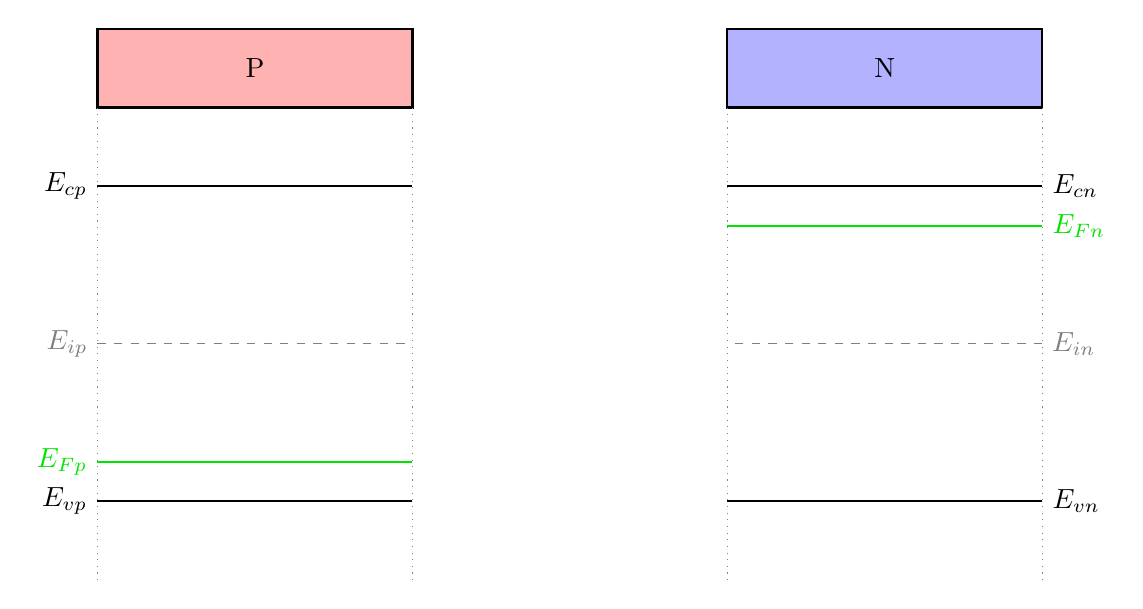
\begin{tikzpicture}
    
\draw[thick,fill=red!30!white]
    (-2,0) coordinate (P1) 
    rectangle
    node[black] {P}
    ++(-4,1) coordinate (P2);

\draw[thick,fill=blue!30!white]
    (+2,0) coordinate (N1) 
    rectangle
    node[black] {N}
    ++(+4,1) coordinate (N2);

\draw[thick] 
(-6,-1) 
coordinate (Ecp)
node[left] {$E_\text{cp}$} --
(Ecp-|P1);

\draw[thick] 
(-6,-5) 
coordinate (Evp)
node[left] {$E_\text{vp}$} --
(Evp-|P1);

\draw[thick,black!10!green] 
(-6,-4.5) 
coordinate (EFp)
node[left] {$E_\text{Fp}$} --
(EFp-|P1);

\draw[dashed,gray]
(-6,-3)
coordinate (Eip)
node[left] {$E_\text{ip}$} --
(Eip-|P1);

%-----------------------------

\draw[thick] 
(+6,-1) 
coordinate (Ecn)
node[right] {$E_\text{cn}$} --
(Ecn-|N1);

\draw[thick] 
(+6,-5) 
coordinate (Evn)
node[right] {$E_\text{vn}$} --
(Evn-|N1);

\draw[thick,black!10!green] 
(+6,-1.5) 
coordinate (EFn)
node[right] {$E_\text{Fn}$} --
(EFn-|N1);

\draw[dashed,gray]
(+6,-3)
coordinate (Ein)
node[right] {$E_\text{in}$} --
(Ein-|N1);

%-----------------------------

\foreach \x in {-6,-2,+2,+6}
{
    \draw[dotted,gray,thin]
    (\x,0) -- (\x,-6);
}

\end{tikzpicture}
\end{document}